\subsection{}

Considering the equation
\begin{equation}
    f(t) = \sin(6 \pi t) + \sin(10 \pi t) + \sin(30 \pi t) + \sin(A \pi t)
\end{equation}

1. For the case of $A=0$, determine the fundamental \emph{period} of $f(t)$.

2. Suggest a value of $A$ that would make the signal non-periodic and state why your choice makes it non-periodic.




\subsection{}

Considering the Fourier coefficients $a_k$, $b_k$, $c_{k}$ and $c_{-k}$ where $k$ is a positive integer greater than 0,

1. What is the relation between $c_{k}$ and $c_{-k}$?

2. Which of the Fourier coefficients $a_k$, $b_k$ and $c_{k}$ can be complex, if any?




\subsection{}

Considering the periodic squarewave described by the function

\begin{equation}
    f(t)=
    \begin{cases}
        3 & \text{for } -\frac{1}{2} < t < \frac{1}{2} \\
        0 & \text{for } \frac{1}{2} < t < \frac{3}{2}
    \end{cases}
\end{equation}

\begin{center}
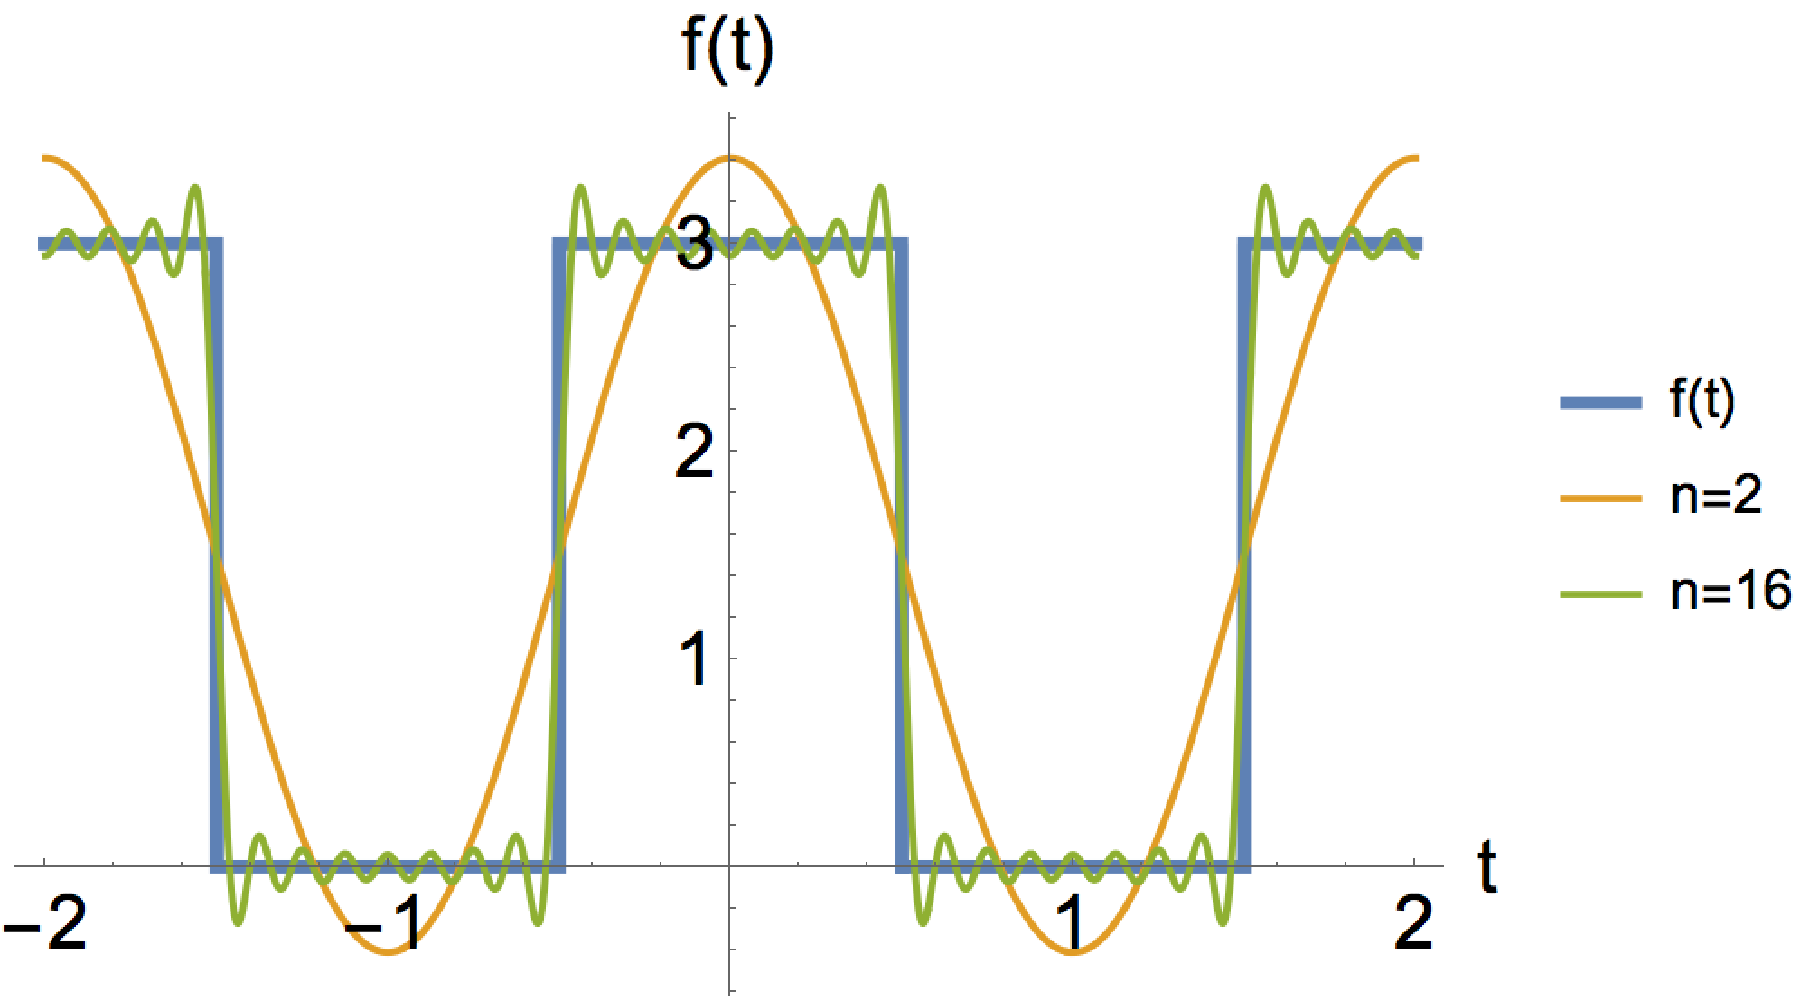
\includegraphics[scale=0.75]{midterm2017-fourier_series_square_wave.png}
\end{center}

1. Obtain the \emph{trigonometric} Fourier series of the above function.

2. What is the common name for a series like the one you have obtained? Why do you obtain a series like this in this situation?

3. What is Gibb's phenomenon? Under what situations does it occur?




\subsection{}

Considering heat on a ring of circumference 1 unit:

1. Write any two possible functions denoting initial temperature distribution on the ring. Please ensure the functional form of each of the two functions is different from the other (ie, you can't just multiply one function by a constant and get the other function). State why you think these functions are valid descriptions of initial temperature distribution.

2. Using any function of initial temperature distribution of your choice (other than the case where the initial temperature is zero everywhere on the ring), obtain an expression for the temperature on the ring at any location and at any time. You will not lose any points for using the simplest possible initial temperature distribution you can imagine (except for zero temperature everywhere on the ring).
